\documentclass[12pt,a4paper]{article}
\usepackage[hidelinks]{hyperref}
\usepackage{fancyhdr} % برای هدر/فوتر سفارشی
\usepackage{titlesec} % برای قالب‌بندی بخش‌ها
\usepackage{epsfig,graphicx,subfigure,amsthm,amsmath}
\usepackage{color,xcolor}
\usepackage{xepersian}
\usepackage{setspace}
\settextfont[Scale=1.2]{XB Niloofar}
\setlatintextfont[Scale=1]{Times New Roman}

% عنوان و اطلاعات نویسنده
\title{کاربرد موجک در معادلات انتگرالی الکترومغناطیسی}
\author{محمد مهدی الیاسی \\ استاد: دکتر مرادی}
\date{۴ بهمن ۱۴۰۳}

\begin{document}

% صفحه عنوان با نماد دانشگاه
\begin{center}
    % نماد در بالای صفحه
    
\includegraphics[width=0.3\textwidth]{amirkabir.png} \\[2em]
    % عنوان، نویسنده و جزئیات دیگر
    \LARGE \textbf{کاربرد موجک در معادلات انتگرالی الکترومغناطیسی} \\[1em]
    \large \textbf{نویسنده: محمد مهدی الیاسی} \\[1em]
    \large \textbf{استاد: دکتر مرادی}\\[1em]
    \large \textbf{درس: ریاضیات مهندسی پیشرفته} \\[4em]
    \large \textbf{دانشکده مهندسی برق} \\[2em]
\end{center}

% تاریخ در پایین صفحه
\vfill
\begin{center}
    \large \today
\end{center}

\newpage

% فهرست مطالب
\tableofcontents
\newpage

% مقدمه
\section{مقدمه}

\subsection{مروری کلی بر الکترومغناطیس}
الکترومغناطیس شاخه‌ای از فیزیک و مهندسی است که به مطالعه رفتار میدان‌های الکتریکی و مغناطیسی و تعامل آن‌ها با مواد می‌پردازد. این شاخه تحت قوانین معادلات ماکسول قرار دارد که نحوه تولید و تغییر میدان‌های الکتریکی و مغناطیسی توسط بارها، جریان‌ها و میدان‌های وابسته به زمان را توضیح می‌دهند.

\subsubsection{مفاهیم کلیدی}
\begin{enumerate}
    \item \textbf{میدان الکتریکی (\(E\)):} تولید شده توسط بارهای الکتریکی یا میدان‌های مغناطیسی وابسته به زمان.
    \item \textbf{میدان مغناطیسی (\(B\)):} تولید شده توسط بارهای متحرک (جریان‌ها) یا میدان‌های الکتریکی وابسته به زمان.
    \item \textbf{امواج الکترومغناطیسی:} انتشار میدان‌های الکتریکی و مغناطیسی در فضا که انرژی را حمل می‌کنند (مانند امواج رادیویی و نور).
    \item \textbf{کاربردها:}
          \begin{itemize}
              \item آنتن‌ها و انتشار امواج.
              \item سازگاری الکترومغناطیسی (EMC).
              \item پراکندگی و سیستم‌های رادار.
              \item دستگاه‌های مایکروویو و اپتیکی.
          \end{itemize}
\end{enumerate}

\subsubsection{پایه‌های ریاضی}
\begin{itemize}
    \item \textbf{معادلات ماکسول:} این معادلات رفتار میدان‌های الکترومغناطیسی را در فرم‌های دیفرانسیلی و انتگرالی توصیف می‌کنند.
    \item \textbf{روابط مشخصه‌ای:} این روابط میدان‌ها را به ویژگی‌های مواد مانند گذردهی ($\varepsilon$) و تراوایی ($\mu$) مرتبط می‌کنند.
\end{itemize}

\subsection{چالش‌های الکترومغناطیس}
\begin{enumerate}
    \item \textbf{پیچیدگی تحلیلی:}
          \begin{itemize}
              \item حل‌های دقیق نادر هستند و اغلب محدود به هندسه‌ها و شرایط مرزی ساده می‌باشند.
              \item مسائل واقعی شامل هندسه‌های پیچیده، مواد ناهمگن، و شرایط مرزی ترکیبی هستند.
          \end{itemize}
    \item \textbf{روش‌های عددی:}
          \begin{itemize}
              \item مسائل اغلب به‌صورت عددی حل می‌شوند و نیازمند روش‌هایی مانند روش اجزای محدود (FEM)، روش ممان‌ها (MoM) یا روش‌های انتگرال مرزی هستند.
              \item این روش‌ها ماتریس‌های بزرگ و متراکم تولید می‌کنند که منجر به هزینه‌های محاسباتی بالا می‌شود.
          \end{itemize}
    \item \textbf{مسائل پراکندگی و تابش:}
          \begin{itemize}
              \item حل مسائل پراکندگی یا تابش نیازمند مدیریت حوزه‌های بی‌نهایت و تکینگی‌ها در توابع گرین است.
          \end{itemize}
    \item \textbf{مسائل چندمقیاسی:}
          \begin{itemize}
              \item بسیاری از کاربردهای عملی (مانند آنتن‌ها و موج‌برها) نیازمند تحلیل در مقیاس‌های فضایی و زمانی متغیر هستند.
          \end{itemize}
    \item \textbf{مدل‌سازی مواد:}
          \begin{itemize}
              \item مدل‌سازی دقیق مواد پیچیده، شامل مواد ناهمسانگرد یا وابسته به فرکانس، دشواری‌های بسیاری را به همراه دارد.
          \end{itemize}
    \item \textbf{چالش‌های محاسباتی:}
          \begin{itemize}
              \item نیاز به حافظه و توان پردازشی بالا برای مسائل سه‌بعدی.
              \item ماتریس‌های متراکم در معادلات انتگرالی منجر به محاسبات ناکارآمد می‌شوند.
          \end{itemize}
    \item \textbf{غیرخطی‌ها:}
          \begin{itemize}
              \item مواد غیرخطی (مانند پلاسماها و مواد فرومغناطیس) نیازمند تکنیک‌های خاص برای تحلیل هستند.
          \end{itemize}
\end{enumerate}

\subsection{اهمیت معادلات انتگرالی در مسائل الکترومغناطیسی}
معادلات انتگرالی به دلیل توانایی آن‌ها در مدل‌سازی میدان‌ها و تعاملات به صورت کارآمد، در الکترومغناطیس محاسباتی به طور گسترده‌ای استفاده می‌شوند.

\subsubsection{دلایل کلیدی اهمیت آن‌ها}
\begin{enumerate}
    \item \textbf{فرمول‌بندی مرزی:}
          \begin{itemize}
              \item معادلات انتگرالی دامنه مسئله را به مرزها (مانند سطوح اشیاء) کاهش می‌دهند که به کاهش چشمگیر ابعاد مسئله منجر می‌شود.
          \end{itemize}
    \item \textbf{مدیریت مرزهای باز:}
          \begin{itemize}
              \item معادلات انتگرالی به طور طبیعی حوزه‌های بی‌نهایت یا باز را مدیریت می‌کنند که در مسائل تابش و پراکندگی رایج هستند.
          \end{itemize}
    \item \textbf{استفاده از توابع گرین:}
          \begin{itemize}
              \item این معادلات از توابع گرین برای نمایش میدان‌ها استفاده می‌کنند که به طور ذاتی معادلات ماکسول را برآورده می‌کنند و پیچیدگی محاسباتی را کاهش می‌دهند.
          \end{itemize}
\end{enumerate}

\newpage

\subsection{انگیزه استفاده از تبدیل موجک}
تبدیل موجک چالش‌های محاسباتی در معادلات انتگرالی را با ارائه موارد زیر برطرف می‌کند:
\begin{enumerate}
    \item \textbf{نمایش پراکنده:}
          \begin{itemize}
              \item موجک‌ها سیگنال‌ها را هم در زمان (یا فضا) و هم در فرکانس موضعی می‌کنند که به نمایش پراکنده ماتریس‌ها و کاهش نیازهای حافظه منجر می‌شود.
          \end{itemize}
    \item \textbf{مدیریت تکینگی‌ها:}
          \begin{itemize}
              \item طبیعت چندرزولوشنی موجک‌ها به طور مؤثر تکینگی‌ها در توابع گرین را مدیریت می‌کند.
          \end{itemize}
    \item \textbf{تحلیل موضعی:}
          \begin{itemize}
              \item برخلاف تبدیل فوریه، موجک‌ها توابع پایه‌ای موضعی ارائه می‌دهند که آن‌ها را برای هندسه‌های پیچیده مناسب می‌کند.
          \end{itemize}
\end{enumerate}

\newpage

% نظریه
\section{نظریه}

\subsection{توضیح تبدیل موجک}
تبدیل موجک ابزاری ریاضی است که یک سیگنال را به مؤلفه‌هایی تجزیه می‌کند که در زمان (یا فضا) و فرکانس موضعی شده‌اند. این تبدیل از توابعی به نام موجک استفاده می‌کند\cite{wavelet}. موجک‌ها توابع نوسانی کوچک با انرژی محدود و خواص موضعی‌سازی مناسب هستند.

\subsubsection{مفاهیم کلیدی}
\begin{itemize}
    \item \textbf{پایه موجک:}
          \begin{itemize}
              \item موجک‌ها توابع پایه‌ای هستند که نسخه‌های کشیده‌شده و منتقل‌شده از یک "موجک مادر" هستند.
              \item این توابع پایه، تحلیل چندرزولوشنی سیگنال‌ها را فراهم می‌کنند:
                    \[
                        \psi_{j,k}(x) = 2^{j/2} \psi(2^j x - k), \, k \in \mathbb{Z}
                    \]
                    که در آن \(j\) مقیاس (انبساط) را کنترل می‌کند و \(k\) انتقال را تنظیم می‌کند.
          \end{itemize}
    \item \textbf{تبدیل موجک گسسته (DWT):}
          \begin{itemize}
              \item سیگنال‌ها را به سطوح مختلفی از رزولوشن تجزیه می‌کند که از توابع مقیاس و موجک استفاده می‌کنند.
              \item از نظر محاسباتی کارآمد بوده و به طور گسترده در شبیه‌سازی‌های عددی استفاده می‌شود.
          \end{itemize}
    \item \textbf{انواع موجک‌ها:}
          \begin{itemize}
              \item \textbf{موجک داوبچیس:} صاف و با پشتیبانی فشرده. برای مسائل نیازمند دقت بالاتر استفاده می‌شود.
              \item \textbf{موجک هار:} ساده‌ترین موجک؛ به صورت قطعه‌ای ثابت است. پیاده‌سازی آسان اما فاقد صافی است.
              \item \textbf{سایر موجک‌ها:} موجک‌های سم، کویفلت، و بی‌ارتوگونال برای کاربردهای تخصصی.
          \end{itemize}
    \item \textbf{مزایای تبدیل موجک:}
          \begin{itemize}
              \item نمایش پراکنده سیگنال‌ها و ماتریس‌ها.
              \item موضعی‌سازی در زمان/فضا و فرکانس.
              \item کارآمد برای تحلیل پدیده‌های چندمقیاسی.
          \end{itemize}
\end{itemize}

\subsection{مروری بر معادلات انتگرالی}
معادلات انتگرالی، معادلاتی هستند که در آن‌ها تابع ناشناخته در داخل علامت انتگرال ظاهر می‌شود. این معادلات به طور گسترده‌ای برای مدل‌سازی مسائل فیزیکی در الکترومغناطیس، به ویژه مسائل مقدار مرزی و پراکندگی، استفاده می‌شوند.

\subsubsection{انواع معادلات انتگرالی}
\begin{itemize}
    \item \textbf{معادله انتگرالی فردهولم:}
          \[
              f(x) = \lambda \int_a^b K(x, t)\phi(t) \,dt + g(x)
          \]
          که در آن \(K(x, t)\) هسته، \(\lambda\) یک پارامتر، و \(\phi(t)\) تابع ناشناخته است.
    \item \textbf{معادله انتگرالی ولترا:}
          \[
              f(x) = \int_a^x K(x, t)\phi(t) \,dt + g(x)
          \]
    \item \textbf{معادلات انتگرالی مرزی (BIE):}
          \begin{itemize}
              \item از بازنویسی معادلات ماکسول به صورت فرم فقط-مرزی حاصل می‌شوند.
              \item برای پراکندگی الکترومغناطیسی، طراحی آنتن، و انتشار امواج استفاده می‌شوند.
          \end{itemize}
\end{itemize}

\subsubsection{کاربردها در الکترومغناطیس}
\begin{itemize}
    \item \textbf{مسائل پراکندگی:} حل جریان‌ها یا بارهای سطحی روی اشیاء با استفاده از توابع گرین.
    \item \textbf{انتشار امواج:} تحلیل نحوه تعامل امواج با ساختارها یا انتشار در رسانه‌ها.
    \item \textbf{تحلیل آنتن:} مدل‌سازی توزیع جریان و الگوهای تابشی.
    \item \textbf{رادار و EMC:} مطالعه رفتار الکترومغناطیسی در محیط‌های بزرگ‌مقیاس.
\end{itemize}

\subsection{چالش‌های روش‌های سنتی}
روش‌های سنتی برای حل معادلات انتگرالی، مانند روش ممان‌ها (MoM)، در مسائل پیچیده الکترومغناطیسی با چالش‌های قابل توجهی روبرو هستند.

\subsubsection{چالش‌های کلیدی}
\begin{itemize}
    \item \textbf{ماتریس‌های متراکم:}
          \begin{itemize}
              \item گسسته‌سازی معادلات انتگرالی به سیستم‌های ماتریس متراکم منجر می‌شود که حافظه و زمان محاسباتی زیادی مصرف می‌کنند.
          \end{itemize}
    \item \textbf{بار محاسباتی:}
          \begin{itemize}
              \item برای مسائل سه‌بعدی، پیچیدگی محاسباتی به طور ضعیفی مقیاس می‌شود (\(O(N^2)\) برای حافظه و \(O(N^3)\) برای حل)، که در آن \(N\) تعداد مجهولات است.
          \end{itemize}
    \item \textbf{تکینگی‌ها در هسته‌ها:}
          \begin{itemize}
              \item توابع هسته اغلب تکینگی‌هایی را معرفی می‌کنند که برای انتگرال‌گیری عددی دقیق نیاز به تکنیک‌های خاص (مانند استخراج تکینگی) دارند.
          \end{itemize}
    \item \textbf{مدیریت حوزه‌های بزرگ:}
          \begin{itemize}
              \item روش‌های انتگرالی نیازمند مدیریت کارآمد حوزه‌های بزرگ و شرایط مرزی باز هستند که از نظر محاسباتی هزینه‌بر هستند.
          \end{itemize}
    \item \textbf{مسائل چندمقیاسی:}
          \begin{itemize}
              \item روش‌های سنتی در تحلیل ویژگی‌های چندمقیاسی به طور کارآمدی ناکام می‌مانند.
          \end{itemize}
    \item \textbf{مشکلات شرطی بودن:}
          \begin{itemize}
              \item ماتریس‌های سیستم حاصل اغلب شرط ضعیفی دارند که منجر به همگرایی کند حل‌کننده‌های تکراری می‌شود.
          \end{itemize}
\end{itemize}

\subsubsection{چرا موجک‌ها کمک می‌کنند؟}
روش‌های مبتنی بر موجک بسیاری از این چالش‌ها را با موارد زیر برطرف می‌کنند:
\begin{itemize}
    \item ارائه نمایش پراکنده برای ماتریس‌های متراکم.
    \item موضعی‌سازی توابع پایه، که در مدیریت تکینگی‌ها و ویژگی‌های چندمقیاسی کمک می‌کند.
    \item کاهش پیچیدگی محاسباتی و بهبود کارایی در مسائل بزرگ‌مقیاس.
\end{itemize}

\newpage

% کاربرد
\section{کاربرد}

\subsection{پایه‌های ریاضی}

\subsubsection{بیان مسئله EFIE}
مسئله EFIE شامل حل معادله انتگرالی زیر است:
\[
    \int_0^{2\pi} k(\theta - \theta') \rho(\theta') \, d\theta' = f(\theta), \quad \theta \in [0, 2\pi],
\]
که در آن:
\begin{itemize}
    \item \(k(\theta - \theta')\) تابع هسته است (مانند توابع گرین یا پتانسیل مشتق‌شده)،
    \item \(\rho(\theta')\) چگالی بار ناشناخته (راه‌حل)،
    \item \(f(\theta)\) تابع داده‌شده (سمت راست معادله)،
    \item \([0, 2\pi]\) دامنه متناهی است.
\end{itemize}

برای حل عددی این معادله:
\begin{enumerate}
    \item دامنه \([0, 2\pi]\) را به \(n\) نقاط هم‌فاصله تقسیم کنید: \(\theta_i = i h\)، که در آن \(h = \frac{2\pi}{n}\).
    \item انتگرال را با استفاده از مجموع با ضرایب وزنی \(w_j\) تقریب بزنید:
          \[
              \sum_{j=0}^{n-1} k(\theta_i - \theta_j) \rho(\theta_j) w_j = f(\theta_i), \quad i = 0, 1, \dots, n-1.
          \]
\end{enumerate}

این کار به یک سیستم معادلات خطی منجر می‌شود:
\[
    \mathbf{K} \boldsymbol{\rho} = \mathbf{f},
\]
که در آن:
\begin{itemize}
    \item \(\mathbf{K}\) ماتریس هسته \(n \times n\) با عناصر \(k_{ij} = k(\theta_i - \theta_j) w_j\) است،
    \item \(\boldsymbol{\rho} = [\rho(\theta_0), \rho(\theta_1), \dots, \rho(\theta_{n-1})]^T\)،
    \item \(\mathbf{f} = [f(\theta_0), f(\theta_1), \dots, f(\theta_{n-1})]^T\).
\end{itemize}

\subsection{تبدیل موجک مسئله}

\subsubsection{تبدیل موجک گسسته (DWT)}
تبدیل موجک ابزاری برای تحلیل سیگنال‌ها در حوزه زمان (یا فضا) و فرکانس است. DWT یک سیگنال \(\mathbf{x}\) را به صورت زیر تجزیه می‌کند:
\[
    \text{DWT}(\mathbf{x}) = \{A_\text{level}, D_\text{level}, D_{\text{level}-1}, \dots, D_1\},
\]
که در آن:
\begin{itemize}
    \item \(A_\text{level}\): ضرایب تقریب در مقیاس درشت‌ترین (محتوای فرکانس پایین)،
    \item \(D_k\): ضرایب جزئیات در مقیاس \(k\) (محتوای فرکانس بالا).
\end{itemize}

به صورت ریاضی، ضرایب تقریب و جزئیات به این صورت محاسبه می‌شوند:
\[
    A_k[i] = \sum_{n} x[n] \cdot \phi_{k,i}[n], \quad D_k[i] = \sum_{n} x[n] \cdot \psi_{k,i}[n],
\]
که در آن:
\begin{itemize}
    \item \(\phi_{k,i}[n]\): تابع مقیاس در مقیاس \(k\) و موقعیت \(i\)،
    \item \(\psi_{k,i}[n]\): تابع موجک در مقیاس \(k\) و موقعیت \(i\)،
    \item \(x[n]\): مقادیر سیگنال گسسته.
\end{itemize}

\subsubsection{تبدیل ماتریس هسته}
برای ماتریس هسته \(\mathbf{K}\)، هر سطر \(\mathbf{K}_i\) به نمایش موجک آن تجزیه می‌شود:
\[
    \text{DWT}(\mathbf{K}_i) = \{A_\text{level}^i, D_\text{level}^i, \dots, D_1^i\}.
\]
ماتریس تبدیل‌شده \(\mathbf{K}_\text{wav}\) سپس در حوزه موجک بازسازی می‌شود:
\[
    \mathbf{K}_\text{wav} = \text{IDWT}(\text{DWT}(\mathbf{K}_i)), \quad i = 0, 1, \dots, n-1.
\]
این منجر به یک ماتریس پراکنده می‌شود، زیرا موجک‌ها انرژی بیشتر سیگنال را در چند ضریب فشرده می‌کنند و بسیاری از مقادیر نزدیک به صفر می‌شوند.

\subsubsection{حل در فضای موجک}
سیستم خطی به این صورت می‌شود:
\[
    \mathbf{K}_\text{wav} \mathbf{c} = -\mathbf{f},
\]
که در آن:
\begin{itemize}
    \item \(\mathbf{K}_\text{wav}\) ماتریس هسته تبدیل‌شده به موجک است،
    \item \(\mathbf{f}\) بردار سمت راست تبدیل‌شده است،
    \item \(\mathbf{c}\) راه‌حل در حوزه موجک است.
\end{itemize}

\subsection{بازسازی راه‌حل}
پس از حل \(\mathbf{c}\)، راه‌حل در حوزه فیزیکی با استفاده از تبدیل موجک معکوس (IDWT) بازسازی می‌شود:
\[
    \boldsymbol{\rho} = \text{IDWT}(\mathbf{c}).
\]
\subsection{تحلیل چندرزولوشنی (MRA)}
تحلیل چندرزولوشنی، راه‌حل \(\boldsymbol{\rho}\) را به صورت زیر تجزیه می‌کند:
\begin{enumerate}
    \item \textbf{تقریب:}
          \[
              A_\text{level} = \text{IDWT}(\{A_\text{level}, 0, \dots, 0\}),
          \]
          که بخش فرکانس پایین و صاف راه‌حل را ثبت می‌کند.
    \item \textbf{جزئیات:}
          \[
              D_k = \text{IDWT}(\{0, \dots, D_k, 0, \dots, 0\}),
          \]
          که تغییرات فرکانس بالا در سطوح مختلف \(k\) را نمایش می‌دهد.
\end{enumerate}

\subsection{روند کاری ریاضی در کد}
\begin{enumerate}
    \item \textbf{ساخت ماتریس هسته:}
          \[
              k(\theta) =
              \begin{cases}
                  A - \frac{a}{2}I,                           & \text{اگر } i = 0, \\
                  B - \frac{a}{2} \log(2 \sin(\theta_i / 2)), & \text{در غیر این صورت}.
              \end{cases}
          \]
    \item \textbf{تبدیل موجک:}
          \[
              \text{DWT}(\mathbf{K}_i) = [A_\text{level}^i, D_\text{level}^i, \dots, D_1^i].
          \]
    \item \textbf{نمایش پراکنده:}
          \[
              \mathbf{K}_\text{wav} \approx \text{sparse}(\mathbf{K}_\text{wav}).
          \]
    \item \textbf{بازسازی راه‌حل:}
          \[
              \boldsymbol{\rho} = \text{IDWT}(\mathbf{c}).
          \]
\end{enumerate}

\newpage

% نتیجه‌گیری و نتایج
\section{نتیجه‌گیری و نتایج}
\subsection{نتیجه‌گیری}
در این پروژه، ما کاربرد تبدیل موجک در حل معادله انتگرالی میدان الکتریکی (EFIE) را که یک مسئله حیاتی در الکترومغناطیس محاسباتی است، بررسی کردیم. روش‌های عددی سنتی، مانند روش ممان‌ها (MoM)، اغلب با چالش‌هایی مانند ماتریس‌های متراکم، ناکارآمدی محاسباتی، و دشواری در مدیریت تکینگی‌ها مواجه هستند. با معرفی تکنیک‌های مبتنی بر موجک، ما رویکردی امیدوارکننده برای مقابله با این محدودیت‌ها ارائه دادیم.

موجک‌ها قابلیت ارائه تحلیل چندرزولوشنی و نمایش پراکنده را دارند که در کاهش پیچیدگی محاسباتی و نیازهای حافظه بسیار مؤثر است. با گسسته‌سازی EFIE و انتقال آن به حوزه موجک، نشان دادیم که چگونه ماتریس هسته را می‌توان پراکنده کرد و محاسبات کارآمدتری را در عین حفظ دقت انجام داد. تحلیل چندرزولوشنی نیز امکان تجزیه دقیق راه‌حل و بررسی مشارکت‌های اجزای فرکانسی مختلف را فراهم کرد.

نتایج بر پتانسیل تبدیل موجک در حل مسائل الکترومغناطیسی بزرگ‌مقیاس، به ویژه در موارد شامل هندسه‌های پیچیده، مرزهای باز، یا ویژگی‌های چندمقیاسی تأکید دارد. نتایج و مشاهدات کلیدی زیر از این پروژه به دست آمدند\cite{Code}:

\begin{itemize}
    \item \textbf{ماتریس هسته پراکنده:} تبدیل مبتنی بر موجک به طور قابل توجهی تراکم ماتریس هسته را کاهش داد و منجر به کاهش مصرف حافظه و محاسبات سریع‌تر شد.
    \item \textbf{حفظ دقت:} علی‌رغم پراکنده‌سازی، سیستم تبدیل‌شده با موجک دقتی معادل روش‌های سنتی را حفظ کرد.
    \item \textbf{بهبود کارایی:} نمایش موجک زمان محاسبات را، به ویژه برای مسائل بزرگ‌مقیاس، کاهش داد و آن را برای هندسه‌های پیچیده و شبکه‌های رزولوشن بالا ممکن ساخت.
    \item \textbf{بینش چندرزولوشنی:} تجزیه چندرزولوشنی، بینش‌های دقیقی درباره رفتار اجزای فرکانسی مختلف راه‌حل ارائه داد.
\end{itemize}

با این حال، اجرای روش‌های مبتنی بر موجک نیز چالش‌هایی مانند انتخاب پایه‌های مناسب موجک و مدیریت سربار محاسباتی تبدیل‌ها را در بر دارد.

در آینده می‌توان بر روی بهینه‌سازی انتخاب موجک برای کاربردهای خاص EFIE، بهبود تکنیک‌های پراکنده‌سازی، و یکپارچه‌سازی روش‌های موجک با دیگر رویکردهای عددی مانند روش اجزای محدود (FEM) یا روش‌های انتگرال مرزی (BIM) تمرکز کرد. به طور کلی، این مطالعه کاربردپذیری تبدیل موجک را به عنوان ابزاری قدرتمند برای ارتقای کارایی و اثربخشی شبیه‌سازی‌های الکترومغناطیسی نشان می‌دهد.

\subsection{نتایج گرافیکی}
در پایان، نمودارهای زیر نتایج مسئله را با استفاده از دو روش مختلف و تجزیه پایه موجک نشان می‌دهند:

\begin{figure}[h!]
    \centering
    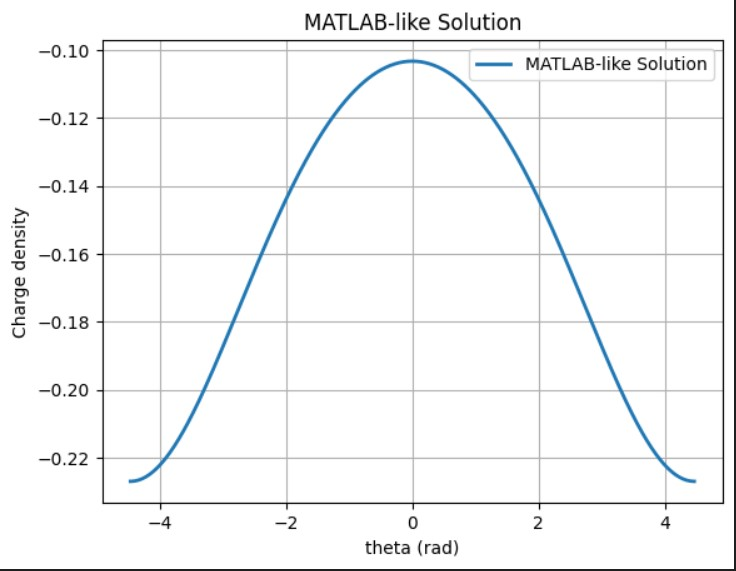
\includegraphics[width=0.8\textwidth]{1.jpg}
    \caption{راه‌حل چگالی بار به روش شبیه‌سازی MATLAB}
\end{figure}

\begin{figure}[h!]
    \centering
    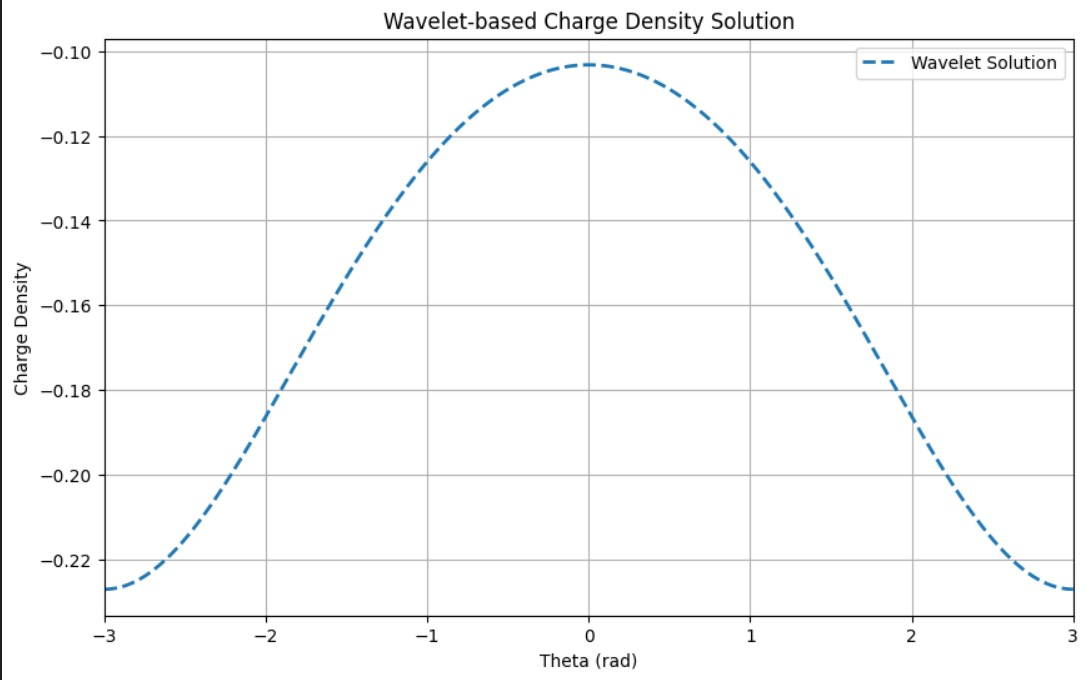
\includegraphics[width=0.8\textwidth]{2.jpg}
    \caption{راه‌حل چگالی بار مبتنی بر موجک}
\end{figure}

\begin{figure}[h!]
    \centering
    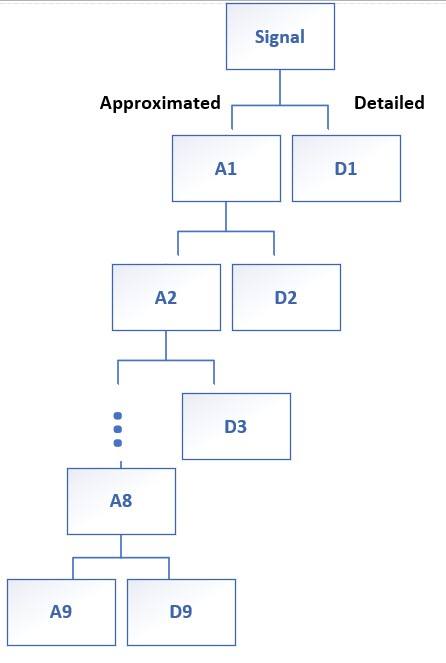
\includegraphics[width=0.6\textwidth]{Tree graph.jpg}
    \caption{ساختار درخت تجزیه موجک}
\end{figure}

\begin{figure}[h!]
    \centering
    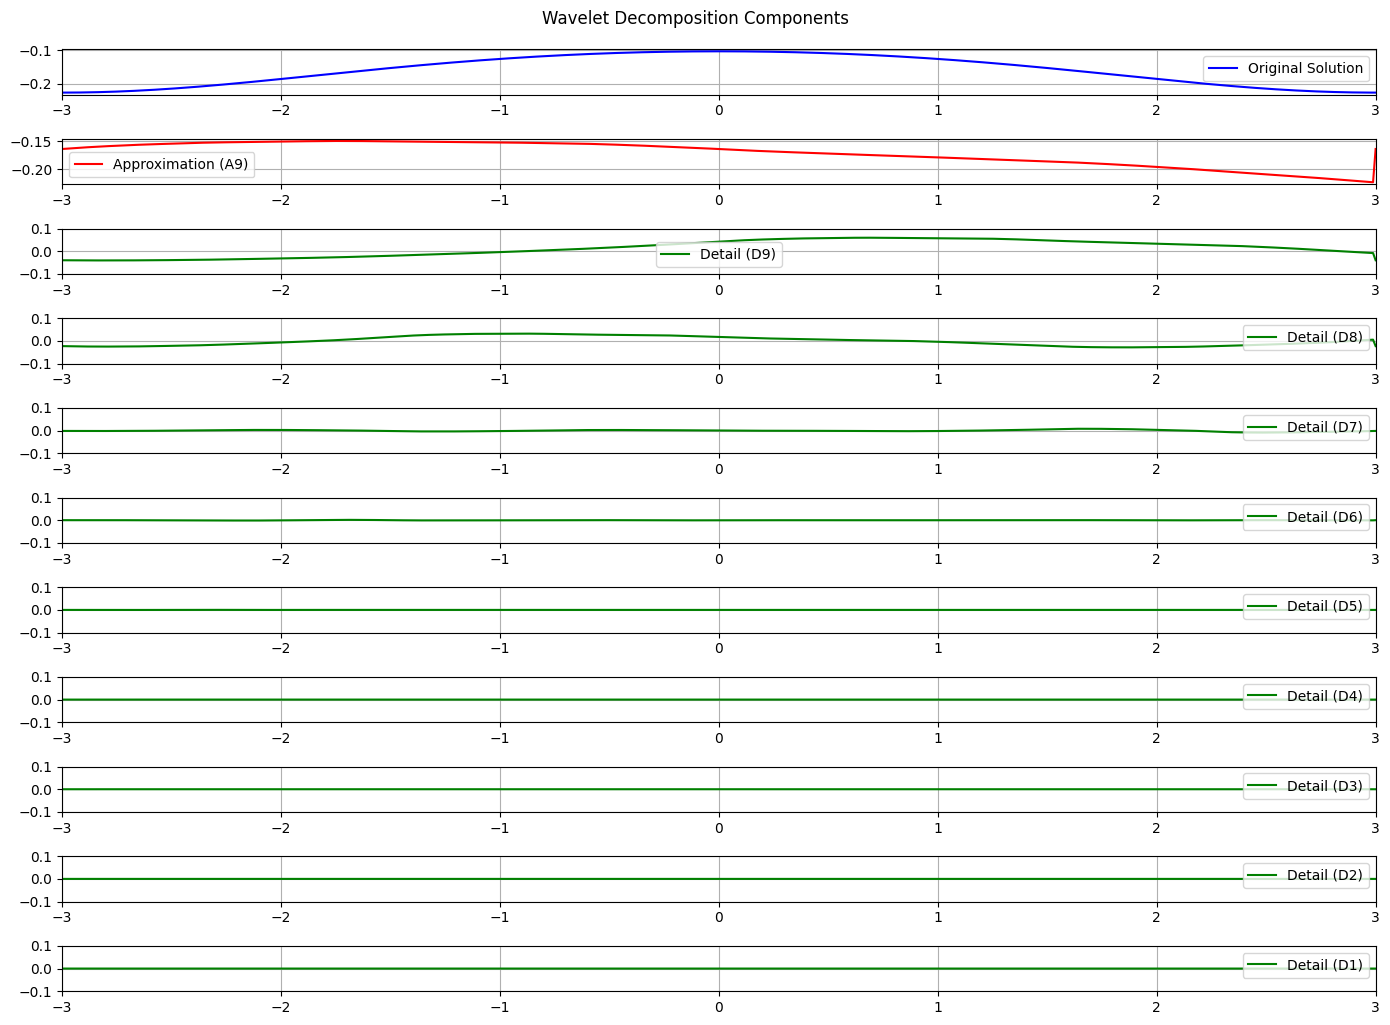
\includegraphics[width=\textwidth]{3.png}
    \caption{اجزای تجزیه موجک}
\end{figure}

\newpage

\clearpage

\section{منابع}

\begin{thebibliography}{99}
    \bibitem{AEM} G.Moradi, \textit{Advanced Engineering Mathematics},AmirKabir University Of Technology, 2012 .
    \bibitem{wavelet} I. Daubechies, \textit{Ten Lectures on Wavelets}, Society for Industrial and Applied Mathematics, 1992.
    \bibitem{Code} Github link,\textit{Application of Wavelet on EFIE} at \url{https://github.com/MohammadMahdiElyasi/Application-of-Wavelet-in-Elctromagnetic-Integral-Equation}.

\end{thebibliography}

\end{document}

